\section{Motivation}

\begin{frame}{Same Weights, 74\% or 93\%}
    \begin{columns}[T,onlytextwidth]
        \column{0.62\textwidth}
        \begin{itemize}\itemsep0.55em
            \item OpenAI's o1 on AIME 2024 mathematics problems. GPT-4o solves 12\%. o1 solves \textbf{74\% to 93\%, depending on inference settings}.
            \item The ladder: 74\% with one sample, 83\% with a vote over 64 samples, 93\% when a learned scorer re-ranks 1,000 samples.
            \item Nothing in the model changed between those three numbers. What changed is \alert{how many candidates were generated} and \alert{what chose among them}.
            \item One reading: test-time scaling is ``a new axis for scaling compute''. The plot on the right is linear in the \emph{logarithm} of compute, so each constant gain costs a multiple.
        \end{itemize}
        \column{0.35\textwidth}
        \centering
        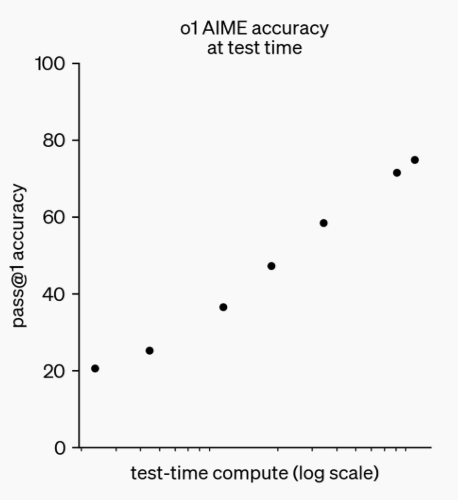
\includegraphics[width=\linewidth,height=0.62\textheight,keepaspectratio]{images/advanced-reasoning/metacot_o1_inference.png}
    \end{columns}
    \vspace{0.2em}
    \src{Range and GPT-4o baseline: Wolfe, ``Demystifying Reasoning Models'' (Feb 2025). Per-setting ladder: OpenAI, ``Learning to reason with LLMs'' (Sep 2024). Quote: Hoogland, ``o1: A Technical Primer'' (Dec 2024). Plot: OpenAI's o1 launch figure as reproduced in Xiang et al., \href{https://arxiv.org/abs/2501.04682}{arXiv:2501.04682}, Figure 9.}
\end{frame}

\begin{frame}{One Idea, Told Ten Times}
    \begin{itemize}\itemsep0.4em
        \item Every method today has the same two parts: \textbf{generate} candidates, then \textbf{select or correct} them.
        \item Generation is cheap to scale. The question is always what does the selecting.
    \end{itemize}
    \begin{center}
    \small
    \renewcommand{\arraystretch}{1.15}
    \begin{adjustbox}{max width=\linewidth}\begin{tabular}{>{\raggedright\arraybackslash}p{4.2cm}>{\raggedright\arraybackslash}p{4.6cm}>{\raggedright\arraybackslash}p{4.6cm}}
        \toprule
        \textbf{The checker is} & \textbf{Examples} & \textbf{What happens as compute grows} \\
        \midrule
        \rowcolor{KAUSTcyan!12} \textbf{Exact} & unit tests, Lean, a classical planner, a robust answer grader & coverage turns into accuracy. Search works \\
        \textbf{A model} & a reward model, an LLM judge, the model's own critique & gains plateau, over-optimise, or get hacked \\
        \bottomrule
    \end{tabular}\end{adjustbox}
    \end{center}
    \begin{itemize}\itemsep0.4em
        \item The 2025 to 2026 shift: the industry moved the checker \emph{inside training} and left the user an \textbf{effort dial}.
    \end{itemize}
    \vspace{0.1em}
    \takeaway{Compute spent at inference is only as useful as the signal that selects or corrects what it produces.}
\end{frame}

\begin{frame}{Today's Map: One Loop, Ten Questions}
    \centering
    \begin{adjustbox}{max width=\linewidth}\begin{tikzpicture}[font=\small,
        blk/.style={draw, rounded corners=2pt, minimum width=3.0cm, minimum height=0.8cm, align=center},
        note/.style={align=left, text width=4.1cm, font=\footnotesize},
        arr/.style={-{Stealth}, thick, KAUSTblue}]
        \node[blk, fill=KAUSTcyan!20] (gen) at (0,3.6) {\textbf{Generate}};
        \node[blk, fill=darkorange!20] (ver) at (0,1.8) {\textbf{Verify and select}};
        \node[blk, fill=gray!12] (rev) at (0,0) {\textbf{Revise and plan}};
        \draw[-{Stealth}, thick] (gen) -- (ver);
        \draw[-{Stealth}, thick] (ver) -- (rev);
        \draw[-{Stealth}, thick] (rev.west) to[out=180, in=180, looseness=1.2] (gen.west);
        \draw[dashed, gray] (-2.6,-0.75) rectangle (2.0,4.35);
        \node[font=\scriptsize, gray] at (0,-1.0) {9. can the whole loop be learned?};
        \node[note, anchor=west] (n1) at (2.5,4.1) {\textbf{1. How does thinking scale?}\\Test-time compute};
        \node[note, anchor=west] (n2) at (2.5,3.1) {\textbf{2, 3. How to structure it?}\\Chains, trees, graphs, search};
        \node[note, anchor=west] (n4) at (2.5,2.0) {\textbf{4. What scores a step?}\\Process and outcome rewards};
        \node[note, anchor=west] (n5) at (2.5,0.95) {\textbf{5, 6. Can the check be exact?}\\Code, symbolic tools, Lean};
        \node[note, anchor=east] (n7) at (-3.3,2.6) {\textbf{7. Can a model fix itself?}\\Self-correction and its failures};
        \node[note, anchor=east] (n8) at (-3.3,1.3) {\textbf{8. Can it plan?}\\Planning with a verifier};
        \node[note, anchor=east] (n10) at (-3.3,-0.1) {\textbf{10. Where do models stand?}\\Reasoning paradigms in 2026};
        \draw[arr] (n1.west) -- (gen.east);
        \draw[arr] (n2.west) -- (gen.south east);
        \draw[arr] (n4.west) -- (ver.east);
        \draw[arr] (n5.west) -- (ver.south east);
        \draw[arr] (n7.east) -- (-2.25,2.0);
        \draw[arr] (n8.east) -- (rev.north west);
        \draw[arr] (n10.east) -- (-2.6,-0.1);
    \end{tikzpicture}\end{adjustbox}
\end{frame}
